\chapter{Methodology}
\section{Dataset Preparation}

This study used a publicly available Mango Leaf Disease Dataset from Kaggle, which contains 4,000 images of healthy and diseased mango leaves captured under natural lighting conditions with a uniform background. The dataset includes eight categories: Anthracnose, Bacterial Canker, Cutting Weevil, Die Back, Gall Midge, Powdery Mildew, Sooty Mould and Healthy.\\
All images were visually inspected for quality and resized to a uniform resolution of 224$\times$224 pixels to ensure compatibility across all convolutional neural network (CNN) models. The dataset was then divided into training, validation, and testing subsets using stratified sampling to maintain balanced class representation.

\subsection{Supervised Dataset Preparation}

In the supervised learning setup, all samples were treated as labeled. The dataset was divided into \textbf{80\% for training}, \textbf{10\% for validation}, and \textbf{10\% for testing}, resulting in 3,200, 400, and 400 images, respectively.  

\begin{figure}[H]
\centering
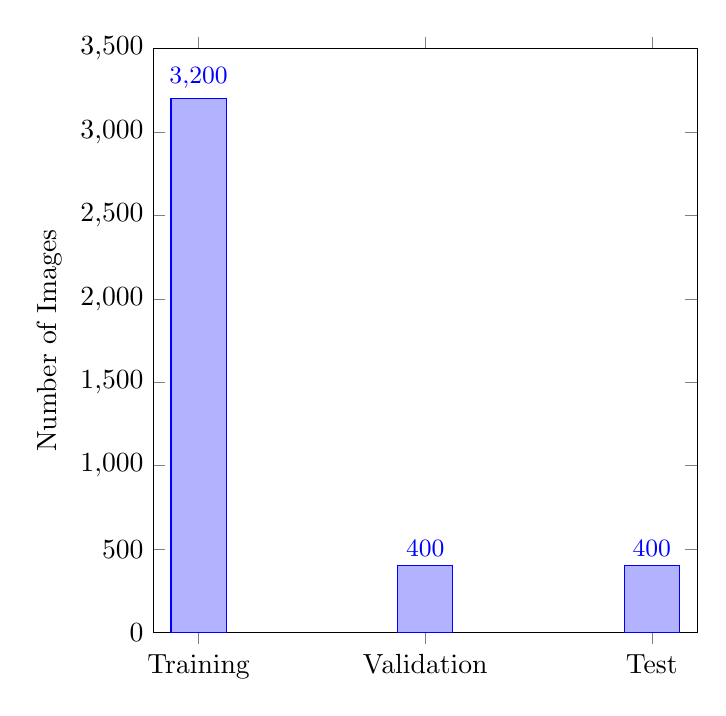
\begin{tikzpicture}
\begin{axis}[
    ybar,
    width=0.7\textwidth,
    height=9cm, % increased height
    bar width=20pt,
    ylabel={Number of Images},
    symbolic x coords={Training, Validation, Test},
    xtick=data,
    nodes near coords,
    every node near coord/.append style={font=\small},
    ymin=0,
    ymax=3500 % optional: make top of axis a bit higher than largest bar
]
\addplot coordinates {(Training,3200) (Validation,400) (Test,400)};
\end{axis}
\end{tikzpicture}
\caption{Supervised dataset split across training, validation, and test sets.}
\label{fig:supervised_split_simple}
\end{figure}
All images were normalized to pixel values between 0 and 1. The validation set was used for model tuning and early stopping, while the test set was used exclusively for the final evaluation. This preprocessing ensured the model was trained on a diverse yet balanced dataset, minimizing overfitting and improving robustness.

\subsection{Semi-Supervised Dataset Preparation}

For the semi-supervised setup, the same dataset was used, but with a reduced number of labeled samples to simulate limited annotation scenarios. From the total dataset, 80\% was used for training, 10\% for validation, and 10\% for testing. Within the training subset, only \textbf{25\% (800 images)} were labeled, while the remaining \textbf{75\% (2,400 images)} were treated as unlabeled. Class balance was maintained within the labeled portion.  

\begin{figure}[H]
\centering
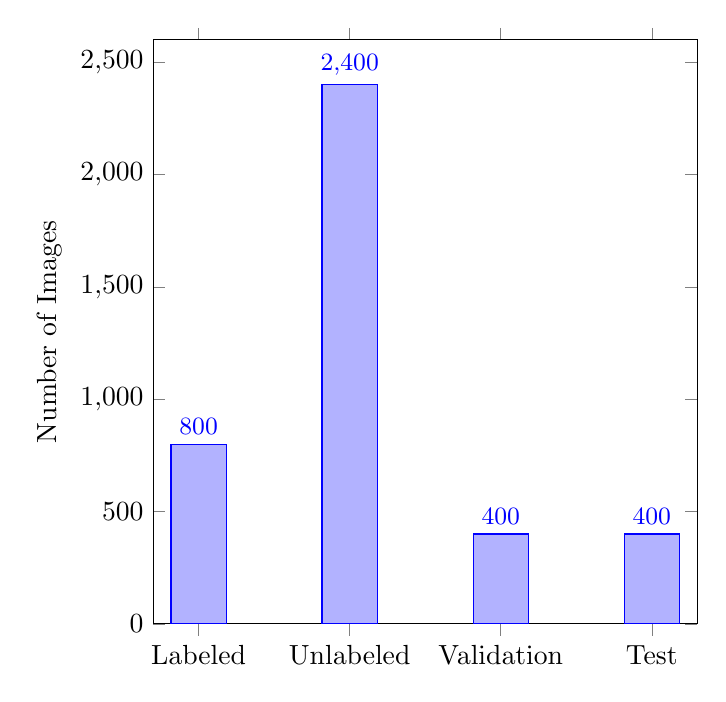
\begin{tikzpicture}
\begin{axis}[
    ybar,
    width=0.7\textwidth,
    height=9cm, % increased height
    bar width=20pt,
    ylabel={Number of Images},
    symbolic x coords={Labeled, Unlabeled, Validation, Test},
    xtick=data,
    nodes near coords,
    every node near coord/.append style={font=\small},
    ymin=0,
    ymax=2600 % slightly higher than the largest bar
]
\addplot coordinates {(Labeled,800) (Unlabeled,2400) (Validation,400) (Test,400)};
\end{axis}
\end{tikzpicture}
\caption{Semi-supervised dataset split showing labeled, unlabeled, validation, and test samples.}
\label{fig:semi_supervised_split_simple}
\end{figure}
The validation and test sets were kept completely separate and were not used during any training phase.


\section{VGG16 Model Architecture with Adapted Dense Layers}

\subsection{Initial Model Configuration}
The VGG16 model is initialized with ImageNet pre-trained weights while excluding the top classification layers. The base model receives input images of size $224 \times 224 \times 3$. To adapt VGG16 for our mango leaf disease classification task, we added custom dense layers on top of the frozen convolutional base:
\begin{itemize}
    \item Global Average Pooling 2D layer to reduce spatial dimensions.
    \item Dense layer with 256 neurons, ReLU activation, and L2 regularization ($0.016$).
    \item Batch Normalization layer for training stability.
    \item Dropout layer (0.5) to prevent overfitting.
    \item Dense layer with 128 neurons, ReLU activation, and L2 regularization ($0.016$).
    \item Dropout layer (0.3) for further regularization.
    \item Output Dense layer with softmax activation for multi-class classification.
\end{itemize}

\begin{figure}[htbp]
\centering
\begin{tikzpicture}[font=\sffamily\footnotesize, node distance=6mm,
layer/.style={rectangle, rounded corners=4pt, draw=black!40,
fill=#1!18, minimum width=4.2cm, minimum height=9mm, align=center},
arrow/.style={->, thick, >=stealth}
]

% Input
\node[layer=blockgray] (input) {Input Image\\(224×224×3)};

% ResNet101
\node[layer=blockblue, below=of input] (resnet)
{Vgg16 Backbone\\(Pretrained on ImageNet)\\\scriptsize include\_top=False};

% Freeze
\node[layer=blockgray, below=of resnet] (freeze)
{Frozen Convolutional Layers};

% GAP Layer
\node[layer=blockorange, below=of freeze] (gap)
{Global Average Pooling};

% Dense 1
\node[layer=blockgreen, below=of gap] (dense1)
{Dense(256) + ReLU\\Dropout(0.5)};

% Dense 2
\node[layer=blockorange, below=of dense1] (dense2)
{Dense(128) + ReLU\\Dropout(0.3)};

% Output
\node[layer=blockblue, below=of dense2] (output)
{Output Dense(8, Softmax)};

% Arrows
\draw[arrow] (input) -- (resnet);
\draw[arrow] (resnet) -- (freeze);
\draw[arrow] (freeze) -- (gap);
\draw[arrow] (gap) -- (dense1);
\draw[arrow] (dense1) -- (dense2);
\draw[arrow] (dense2) -- (output);

\end{tikzpicture}

\caption{Transfer learning model using Vgg16 as the feature extractor.}
\label{fig:resnet101_transfer_learning}
\end{figure}

\subsection{Supervised Training Strategy}
The supervised training was performed using a pre-trained VGG16 backbone with custom dense layers for classification. Let the input images be denoted as $\mathbf{X} \in \mathbb{R}^{H \times W \times C}$, where $H$ and $W$ are the height and width, and $C$ is the number of channels. The target labels are one-hot encoded vectors $\mathbf{Y} \in \{0,1\}^{n_\text{classes}}$. The model outputs predictions $\hat{\mathbf{Y}}$ through the softmax function \cite{wang2018high}:

\[
\hat{y}_i = \frac{e^{z_i}}{\sum_{j=1}^{n_\text{classes}} e^{z_j}}, \quad i = 1,2,\dots,n_\text{classes},
\]
where $z_i$ are the logits from the final dense layer. The training minimizes the \textbf{categorical cross-entropy loss} \cite{zhang2018generalized}:

\[
\mathcal{L}(\mathbf{Y}, \hat{\mathbf{Y}}) = - \sum_{i=1}^{n_\text{classes}} y_i \log(\hat{y}_i).
\]
Initially, the VGG16 base was \textbf{frozen}, and only the added dense layers were trained using the \textbf{Adamax optimizer} with learning rate $\eta = 10^{-3}$. Early stopping with a patience of 10 epochs and model checkpointing were employed to prevent overfitting. To improve generalization, \textbf{dropout} layers and L2 regularization ($\lambda \|\mathbf{W}\|_2^2$) were applied in the dense layers, where $\mathbf{W}$ denotes the layer weights. The training process was monitored using the accuracy metric:
\[
\text{Accuracy} = \frac{\text{Number of correct predictions}}{\text{Total number of predictions}}.
\]
Finally, the model was evaluated on the validation and test sets, and training progress was visualized through plots of loss $\mathcal{L}$ and accuracy across epochs.

\subsection{Semi-supervised Fine-Tuning the Model}
The semi-supervised approach enhances the model by leveraging unlabeled data:
\begin{itemize}
    \item \textbf{Phase 1:} Initial training on only 25\% of the labeled training data, following the same  approach as supervised learning.
    \item \textbf{Pseudo-labeling:} The model trained on limited labeled data is used to generate predictions on the remaining unlabeled data. Samples with prediction confidence above 95\% are added to the training set with their predicted labels.
    \item \textbf{Phase 2:} The model is fine-tuned on the combined dataset (original labeled data + high-confidence pseudo-labeled data). The top 4 layers of VGG16 are unfrozen, and the model is trained with a very low learning rate ($10^{-5}$) for up to 100 epochs with early stopping and learning rate reduction \cite{hady2013semi}.
\end{itemize}

\section{MobileNetV2 Model Architecture with Adapted Dense Layers}

\subsubsection{Initial Model Configuration}
MobileNetV2 is initialized with ImageNet pre-trained weights without its top classification layers. The model accepts $224 \times 224 \times 3$ input images. For our specific task, we added custom dense layers:
\begin{itemize}
    \item Global Average Pooling 2D layer.
    \item Dense layer with 256 neurons, ReLU activation, and L2 regularization ($0.016$).
    \item Batch Normalization layer.
    \item Dropout layer (0.5).
    \item Dense layer with 128 neurons, ReLU activation, and L2 regularization ($0.016$).
    \item Dropout layer (0.3).
    \item Output Dense layer with softmax activation.
\end{itemize}

\begin{figure}[htbp]
\centering
\begin{tikzpicture}[font=\sffamily\footnotesize, node distance=6mm,
layer/.style={rectangle, rounded corners=4pt, draw=black!40,
fill=#1!18, minimum width=4.2cm, minimum height=9mm, align=center},
arrow/.style={->, thick, >=stealth}
]

% Input
\node[layer=blockgray] (input) {Input Image\\(224×224×3)};

% ResNet101
\node[layer=blockblue, below=of input] (resnet)
{MovileNetV2 Backbone\\(Pretrained on ImageNet)\\\scriptsize include\_top=False};

% Freeze
\node[layer=blockgray, below=of resnet] (freeze)
{Frozen Convolutional Layers};

% GAP Layer
\node[layer=blockorange, below=of freeze] (gap)
{Global Average Pooling};

% Dense 1
\node[layer=blockgreen, below=of gap] (dense1)
{Dense(256) + ReLU\\Dropout(0.5)};

% Dense 2
\node[layer=blockorange, below=of dense1] (dense2)
{Dense(128) + ReLU\\Dropout(0.3)};

% Output
\node[layer=blockblue, below=of dense2] (output)
{Output Dense(8, Softmax)};

% Arrows
\draw[arrow] (input) -- (resnet);
\draw[arrow] (resnet) -- (freeze);
\draw[arrow] (freeze) -- (gap);
\draw[arrow] (gap) -- (dense1);
\draw[arrow] (dense1) -- (dense2);
\draw[arrow] (dense2) -- (output);

\end{tikzpicture}

\caption{Transfer learning model using MobileNetV2 as the feature extractor.}
\label{fig:resnet101_transfer_learning}
\end{figure}


\subsection{Supervised Training Strategy}
The supervised training was performed using a pre-trained MobileNetV2 backbone with custom dense layers for classification. Let the input images be denoted as $\mathbf{X} \in \mathbb{R}^{H \times W \times C}$, where $H$ and $W$ are the height and width, and $C$ is the number of channels. The target labels are one-hot encoded vectors $\mathbf{Y} \in \{0,1\}^{n_\text{classes}}$. The model outputs predictions $\hat{\mathbf{Y}}$ through the softmax function:

\[
\hat{y}_i = \frac{e^{z_i}}{\sum_{j=1}^{n_\text{classes}} e^{z_j}}, \quad i = 1,2,\dots,n_\text{classes},
\]
where $z_i$ are the logits from the final dense layer. The training minimizes the \textbf{categorical cross-entropy loss}:

\[
\mathcal{L}(\mathbf{Y}, \hat{\mathbf{Y}}) = - \sum_{i=1}^{n_\text{classes}} y_i \log(\hat{y}_i).
\]
Initially, the MobileNetV2 base was \textbf{frozen}, and only the added dense layers were trained using the \textbf{Adamax optimizer} with learning rate $\eta = 10^{-3}$. Early stopping with a patience of 10 epochs and model checkpointing were employed to prevent overfitting. To improve generalization, \textbf{dropout} layers and L2 regularization ($\lambda \|\mathbf{W}\|_2^2$) were applied in the dense layers, where $\mathbf{W}$ denotes the layer weights. The training process was monitored using the accuracy metric:
\[
\text{Accuracy} = \frac{\text{Number of correct predictions}}{\text{Total number of predictions}}.
\]
Finally, the model was evaluated on the validation and test sets, and training progress was visualized through plots of loss $\mathcal{L}$ and accuracy across epochs.

\subsection{Semi-supervised Fine-Tuning the Model}
The semi-supervised approach for MobileNetV2 follows the same pattern as VGG16:
\begin{itemize}
    \item \textbf{Phase 1:} Initial training on only 25\% of the labeled data with the two-stage approach.
    \item \textbf{Pseudo-labeling:} The model generates predictions on unlabeled data, with high-confidence samples ($\geq$95\%) added to the training set.
    \item \textbf{Phase 2:} Fine-tuning on the combined dataset with the top 20 layers of MobileNetV2 unfrozen, using a very low learning rate ($10^{-5}$) for up to 100 epochs with early stopping and learning rate reduction \cite{hady2013semi}.
\end{itemize}

\section{ResNet101 Model Architecture with Adapted Dense Layers}

\subsection{Initial Model Configuration}
ResNet101 is initialized with ImageNet pre-trained weights, excluding the top classification layers. The model processes $224 \times 224 \times 3$ input images. The custom dense layers added for our task include:
\begin{itemize}
    \item Global Average Pooling 2D layer.
    \item Dense layer with 256 neurons, ReLU activation, and L2 regularization ($0.016$).
    \item Batch Normalization layer.
    \item Dropout layer (0.5).
    \item Dense layer with 128 neurons, ReLU activation, and L2 regularization ($0.016$).
    \item Dropout layer (0.3).
    \item Output Dense layer with softmax activation.
\end{itemize}
\begin{figure}[htbp]
\centering
\begin{tikzpicture}[font=\sffamily\footnotesize, node distance=6mm,
layer/.style={rectangle, rounded corners=4pt, draw=black!40,
fill=#1!18, minimum width=4.2cm, minimum height=9mm, align=center},
arrow/.style={->, thick, >=stealth}
]

% Input
\node[layer=blockgray] (input) {Input Image\\(224×224×3)};

% ResNet101
\node[layer=blockblue, below=of input] (resnet)
{ResNet101 Backbone\\(Pretrained on ImageNet)\\\scriptsize include\_top=False};

% Freeze
\node[layer=blockgray, below=of resnet] (freeze)
{Frozen Convolutional Layers};

% GAP Layer
\node[layer=blockorange, below=of freeze] (gap)
{Global Average Pooling};

% Dense 1
\node[layer=blockgreen, below=of gap] (dense1)
{Dense(256) + ReLU\\Dropout(0.5)};

% Dense 2
\node[layer=blockorange, below=of dense1] (dense2)
{Dense(128) + ReLU\\Dropout(0.3)};

% Output
\node[layer=blockblue, below=of dense2] (output)
{Output Dense(8, Softmax)};

% Arrows
\draw[arrow] (input) -- (resnet);
\draw[arrow] (resnet) -- (freeze);
\draw[arrow] (freeze) -- (gap);
\draw[arrow] (gap) -- (dense1);
\draw[arrow] (dense1) -- (dense2);
\draw[arrow] (dense2) -- (output);

\end{tikzpicture}

\caption{Transfer learning model using ResNet101 as the feature extractor.}
\label{fig:resnet101_transfer_learning}
\end{figure}


\subsection{Supervised Training Strategy}
The supervised training was performed using a pre-trained ResNet101 backbone with custom dense layers for classification. Let the input images be denoted as $\mathbf{X} \in \mathbb{R}^{H \times W \times C}$, where $H$ and $W$ are the height and width, and $C$ is the number of channels. The target labels are one-hot encoded vectors $\mathbf{Y} \in \{0,1\}^{n_\text{classes}}$. The model outputs predictions $\hat{\mathbf{Y}}$ through the softmax function:

\[
\hat{y}_i = \frac{e^{z_i}}{\sum_{j=1}^{n_\text{classes}} e^{z_j}}, \quad i = 1,2,\dots,n_\text{classes},
\]
where $z_i$ are the logits from the final dense layer. The training minimizes the \textbf{categorical cross-entropy loss}:

\[
\mathcal{L}(\mathbf{Y}, \hat{\mathbf{Y}}) = - \sum_{i=1}^{n_\text{classes}} y_i \log(\hat{y}_i).
\]
Initially, the ResNet101 base was \textbf{frozen}, and only the added dense layers were trained using the \textbf{Adamax optimizer} with learning rate $\eta = 10^{-3}$. Early stopping with a patience of 10 epochs and model checkpointing were employed to prevent overfitting. To improve generalization, \textbf{dropout} layers and L2 regularization ($\lambda \|\mathbf{W}\|_2^2$) were applied in the dense layers, where $\mathbf{W}$ denotes the layer weights. The training process was monitored using the accuracy metric:
\[
\text{Accuracy} = \frac{\text{Number of correct predictions}}{\text{Total number of predictions}}.
\]
Finally, the model was evaluated on the validation and test sets, and training progress was visualized through plots of loss $\mathcal{L}$ and accuracy across epochs.
\subsection{Semi-supervised Fine-Tuning the Model}
The semi-supervised approach for ResNet101 follows the same pattern:
\begin{itemize}
    \item \textbf{Phase 1:} Initial training on only 25\% of the labeled data with the two-stage approach.
    \item \textbf{Pseudo-labeling:} The model generates predictions on unlabeled data, with high-confidence samples ($\geq$95\%) added to the training set.
    \item \textbf{Phase 2:} Fine-tuning on the combined dataset with the top 30 layers of ResNet101 unfrozen, using a very low learning rate ($10^{-5}$) for up to 100 epochs with early stopping and learning rate reduction \cite{hady2013semi}.
\end{itemize}

\section{DenseNet121 Model Architecture with Adapted Dense Layers}

\subsection{Initial Model Configuration}
DenseNet121 is initialized with ImageNet pre-trained weights, excluding the top classification layers. The model accepts $224 \times 224 \times 3$ input images. The custom dense layers added for our task include:
\begin{itemize}
    \item Global Average Pooling 2D layer.
    \item Dense layer with 256 neurons, ReLU activation, and L2 regularization ($0.016$).
    \item Batch Normalization layer.
    \item Dropout layer (0.5).
    \item Dense layer with 128 neurons, ReLU activation, and L2 regularization ($0.016$).
    \item Dropout layer (0.3).
    \item Output Dense layer with softmax activation.
\end{itemize}

\begin{figure}[htbp]
\centering
\begin{tikzpicture}[font=\sffamily\footnotesize, node distance=6mm,
layer/.style={rectangle, rounded corners=4pt, draw=black!40,
fill=#1!18, minimum width=4.2cm, minimum height=9mm, align=center},
arrow/.style={->, thick, >=stealth}
]

% Input
\node[layer=blockgray] (input) {Input Image\\(224×224×3)};

% ResNet101
\node[layer=blockblue, below=of input] (resnet)
{DenseNet121 Backbone\\(Pretrained on ImageNet)\\\scriptsize include\_top=False};

% Freeze
\node[layer=blockgray, below=of resnet] (freeze)
{Frozen Convolutional Layers};

% GAP Layer
\node[layer=blockorange, below=of freeze] (gap)
{Global Average Pooling};

% Dense 1
\node[layer=blockgreen, below=of gap] (dense1)
{Dense(256) + ReLU\\Dropout(0.5)};

% Dense 2
\node[layer=blockorange, below=of dense1] (dense2)
{Dense(128) + ReLU\\Dropout(0.3)};

% Output
\node[layer=blockblue, below=of dense2] (output)
{Output Dense(8, Softmax)};

% Arrows
\draw[arrow] (input) -- (resnet);
\draw[arrow] (resnet) -- (freeze);
\draw[arrow] (freeze) -- (gap);
\draw[arrow] (gap) -- (dense1);
\draw[arrow] (dense1) -- (dense2);
\draw[arrow] (dense2) -- (output);

\end{tikzpicture}

\caption{Transfer learning model using DenseNet121 as the feature extractor.}
\label{fig:resnet101_transfer_learning}
\end{figure}



\subsection{Supervised Training Strategy}
The supervised training was performed using a pre-trained DenseNet121 backbone with custom dense layers for classification. Let the input images be denoted as $\mathbf{X} \in \mathbb{R}^{H \times W \times C}$, where $H$ and $W$ are the height and width, and $C$ is the number of channels. The target labels are one-hot encoded vectors $\mathbf{Y} \in \{0,1\}^{n_\text{classes}}$. The model outputs predictions $\hat{\mathbf{Y}}$ through the softmax function \cite{wang2018high}:

\[
\hat{y}_i = \frac{e^{z_i}}{\sum_{j=1}^{n_\text{classes}} e^{z_j}}, \quad i = 1,2,\dots,n_\text{classes},
\]
where $z_i$ are the logits from the final dense layer. The training minimizes the \textbf{categorical cross-entropy loss}:

\[
\mathcal{L}(\mathbf{Y}, \hat{\mathbf{Y}}) = - \sum_{i=1}^{n_\text{classes}} y_i \log(\hat{y}_i).
\]
Initially, the DenseNet121 base was \textbf{frozen}, and only the added dense layers were trained using the \textbf{Adamax optimizer} with learning rate $\eta = 10^{-3}$. Early stopping with a patience of 10 epochs and model checkpointing were employed to prevent overfitting. To improve generalization, \textbf{dropout} layers and L2 regularization ($\lambda \|\mathbf{W}\|_2^2$) were applied in the dense layers, where $\mathbf{W}$ denotes the layer weights. The training process was monitored using the accuracy metric:
\[
\text{Accuracy} = \frac{\text{Number of correct predictions}}{\text{Total number of predictions}}.
\]
Finally, the model was evaluated on the validation and test sets, and training progress was visualized through plots of loss $\mathcal{L}$ and accuracy across epochs.
\subsection{Semi-supervised Fine-Tuning the Model}
The semi-supervised approach for DenseNet121 follows the same pattern:
\begin{itemize}
    \item \textbf{Phase 1:} Initial training on only 25\% of the labeled data with the two-stage approach.
    \item \textbf{Pseudo-labeling:} The model generates predictions on unlabeled data, with high-confidence samples ($\geq$95\%) added to the training set.
    \item \textbf{Phase 2:} Fine-tuning on the combined dataset with the top 15 layers of DenseNet121 unfrozen, using a very low learning rate ($10^{-5}$) for up to 100 epochs with early stopping and learning rate reduction \cite{hady2013semi}.
\end{itemize}

\section{Proposed Model Architecture for Supervised and Semi-supervised Classification}

\subsection{Overall Architecture Design}

The proposed model is a custom Convolutional Neural Network (CNN) comprising four convolutional blocks followed by a classification head. Unlike the pre-trained models (VGG16, ResNet101, MobileNetV2, and DenseNet121) that were originally designed for ImageNet classification, this architecture is specifically tailored for the characteristics of mango leaf disease images, providing a balance between model complexity and computational efficiency while preventing overfitting on limited labeled data.\\
The architecture accepts input images of size 224×224×3 pixels and outputs probability distributions across eight disease classes. The model contains approximately 3.5 million trainable parameters, making it significantly more lightweight than the baseline models while maintaining competitive performance.
\begin{figure}[htbp!]
\centering
\begin{tikzpicture}[font=\sffamily\small
, every node/.style={align=center},
    layer/.style={rectangle, rounded corners=4pt, draw=black!40, fill=#1!18, minimum width=2.8cm, minimum height=7mm, inner sep=3pt, drop shadow={shadow xshift=0.5pt, shadow yshift=-0.5pt}},
    smalllayer/.style={rectangle, rounded corners=4pt, draw=black!30, fill=#1!10, minimum width=2.4cm, minimum height=6mm, inner sep=2pt},
    arrow/.style={->, thick, rounded corners=2pt, >=stealth}
]

% Input
\node (input) [smalllayer={blockgray}] {Input\\(\tiny \texttt{\small 224x224x3})};

% Block 1
\node (b1) [layer={blockblue}, below=5mm of input] {Conv2D(32,3x3)\\BatchNorm\\ReLU\\MaxPool(2x2)\\Dropout(0.2)};

% Block 2
\node (b2) [layer={blockgreen}, below=4mm of b1] {Conv2D(64,3x3)\\BatchNorm\\ReLU\\MaxPool(2x2)\\Dropout(0.3)};

% Block 3
\node (b3) [layer={blockorange}, below=4mm of b2] {Conv2D(128,3x3)\\BatchNorm\\ReLU\\MaxPool(2x2)\\Dropout(0.4)};

% Block 4
\node (b4) [layer={blockblue}, below=4mm of b3] {Conv2D(256,3x3)\\BatchNorm\\ReLU\\MaxPool(2x2)\\Dropout(0.5)};

% Global Pooling & Head
\node (gap) [smalllayer={blockgray}, below=4mm of b4] {GlobalAveragePooling2D};
\node (d1) [smalllayer={blockgreen}, below=4mm of gap] {Dense(256)\\ReLU\\Dropout(0.6)};
\node (d2) [smalllayer={blockorange}, below=4mm of d1] {Dense(128)\\ReLU\\Dropout(0.5)};
\node (out) [smalllayer={blockblue}, below=4mm of d2] {\\Output Dense(8, Softmax)\\};

% Connections
\draw[arrow] (input) -- (b1);
\draw[arrow] (b1) -- (b2);
\draw[arrow] (b2) -- (b3);
\draw[arrow] (b3) -- (b4);
\draw[arrow] (b4) -- (gap);
\draw[arrow] (gap) -- (d1);
\draw[arrow] (d1) -- (d2);
\draw[arrow] (d2) -- (out);

\end{tikzpicture}
\caption{Proposed CNN architecture for mango leaf disease classification.}
\label{fig:cnn_architecture}
\end{figure}

\subsection{Convolutional Block Design}

The proposed architecture consists of four hierarchical convolutional blocks, each following a consistent design pattern. The mathematical formulation of the core convolution operation is:

\subsubsection*{Convolutional Operation:}

The convolution operation at layer $l$ is defined as:

\begin{equation}
z^{[l]} = W^{[l]} * a^{[l-1]} + b^{[l]}
\end{equation}

where $W^{[l]}$ represents the learnable filters, $*$ denotes the convolution operation, $a^{[l-1]}$ is the input activation from the previous layer, and $b^{[l]}$ is the bias term.

\subsubsection*{Block 1 (Input Processing):}
\begin{itemize}
    \item Conv2D layer: 32 filters, 3×3 kernel, same padding, L2 regularization (1e-4)
    \item Batch Normalization layer
    \item ReLU activation
    \item Max Pooling: 2×2 pool size
    \item Dropout: 20\% rate
\end{itemize}

\subsubsection*{Block 2 (Feature Extraction):}
\begin{itemize}
    \item Conv2D layer: 64 filters, 3×3 kernel, same padding, L2 regularization (1e-4)
    \item Batch Normalization layer
    \item ReLU activation
    \item Max Pooling: 2×2 pool size
    \item Dropout: 30\% rate
\end{itemize}

\subsubsection*{Block 3 (Mid-level Features):}
\begin{itemize}
    \item Conv2D layer: 128 filters, 3×3 kernel, same padding, L2 regularization (1e-4)
    \item Batch Normalization layer
    \item ReLU activation
    \item Max Pooling: 2×2 pool size
    \item Dropout: 40\% rate
\end{itemize}

\subsubsection*{Block 4 (High-level Features):}
\begin{itemize}
    \item Conv2D layer: 256 filters, 3×3 kernel, same padding, L2 regularization (1e-4)
    \item Batch Normalization layer
    \item ReLU activation
    \item Max Pooling: 2×2 pool size
    \item Dropout: 50\% rate
\end{itemize}
Each block progressively increases both the number of filters (32→64→128→256) and the dropout rate (0.2→0.3→0.4→0.5), enabling the network to learn increasingly complex features while maintaining strong regularization to prevent overfitting.

\subsection{Activation and Pooling Operations}

\subsubsection{ReLU Activation Function}

The Rectified Linear Unit (ReLU) activation function is applied after batch normalization in each convolutional block \cite{schmidt2020nonparametric}:

\begin{equation}
\text{ReLU}(x) = \max(0, x) = \begin{cases} 
x & \text{if } x > 0 \\
0 & \text{if } x \leq 0
\end{cases}
\end{equation}
ReLU introduces non-linearity while maintaining computational efficiency and mitigating the vanishing gradient problem.

\subsubsection{Max Pooling Operation}

Max pooling with 2×2 window reduces spatial dimensions by selecting the maximum value in each pooling region:

\begin{equation}
y_{i,j} = \max_{(p,q) \in \mathcal{R}_{i,j}} x_{p,q}
\end{equation}
where $\mathcal{R}_{i,j}$ represents the 2×2 pooling region corresponding to output position $(i,j)$.

\subsubsection{Dropout Regularization}

During training, dropout randomly sets a fraction $p$ of neurons to zero:

\begin{equation}
\tilde{a}^{[l]} = a^{[l]} \odot m
\end{equation}

where $m \sim \text{Bernoulli}(1-p)$ is a binary mask, and $\odot$ denotes element-wise multiplication. During inference, activations are scaled by $(1-p)$ to maintain expected values.

\subsection{Classification Head}

Following the convolutional blocks, the classification head processes the extracted features through global average pooling and fully connected layers.

\subsubsection{Global Average Pooling}

For feature maps of spatial dimensions $H \times W$ with $C$ channels, global average pooling computes:

\begin{equation}
\text{GAP}_c = \frac{1}{H \times W}\sum_{i=1}^{H}\sum_{j=1}^{W}x_{i,j,c}
\end{equation}

This reduces each feature map to a single value, resulting in a $C$-dimensional vector (256 dimensions from the final convolutional block).

\subsubsection*{Fully Connected Layers:}
\begin{itemize}
    \item Dense Layer 1: 256 units with ReLU activation and L2 regularization (1e-4)
    \item Dropout: 60\% rate
    \item Dense Layer 2: 128 units with ReLU activation and L2 regularization (1e-4)
    \item Dropout: 50\% rate
    \item Output Layer: 8 units with softmax activation
\end{itemize}

\subsubsection{Softmax Activation Function}

The output layer uses softmax activation to produce probability distributions over the 8 disease classes:

\begin{equation}
\text{softmax}(z_i) = \frac{e^{z_i}}{\sum_{j=1}^{K}e^{z_j}}
\end{equation}

where $K=8$ is the number of disease classes, $z_i$ is the logit for class $i$, and the output represents $P(y=i|x)$, the probability of input $x$ belonging to class $i$.

\subsection{Regularization Strategy}

To address the challenge of overfitting on small datasets, the proposed model incorporates multiple regularization techniques:

\subsubsection{L2 Weight Regularization}

All convolutional and dense layers employ L2 regularization with coefficient 1e-4, which adds a penalty term to the loss function that penalizes large weights and promotes model generalization.

\subsubsection{Progressive Dropout}

Dropout rates increase progressively through the network (20\%→30\%→40\%→50\%→60\%→50\%), with the highest rates applied to the fully connected layers where overfitting is most likely to occur. This stochastic regularization technique forces the network to learn robust features that are not dependent on specific neuron activations.

\subsubsection{Batch Normalization}

Applied after each convolutional layer to normalize activations, stabilize training, and provide mild regularization effects. Batch normalization reduces internal covariate shift and allows for higher learning rates during training.

\subsection{Data Augmentation Strategies}

The model employs aggressive data augmentation techniques specifically designed for leaf disease images to artificially expand the training dataset and improve model generalization.

\subsubsection*{Training Augmentation:}
\begin{itemize}
    \item Rotation: Random rotations up to ±40°
    \item Translation: Horizontal and vertical shifts up to 25\%
    \item Shear transformation: Intensity of 0.2
    \item Zoom: Random zoom in/out up to 25\%
    \item Horizontal flip: Random horizontal flipping (50\% probability)
    \item Vertical flip: Random vertical flipping (50\% probability) - as leaves can appear in any orientation
    \item Brightness adjustment: Random brightness variation between 0.7× and 1.3×
    \item Channel shift: RGB channel intensity shifts up to ±20
    \item Normalization: Pixel values rescaled to [0, 1]
\end{itemize}

\subsubsection*{Validation/Test Augmentation:}
\begin{itemize}
    \item Only pixel normalization (rescaling to [0, 1]) is applied to ensure consistent evaluation.
\end{itemize}

\subsection{Supervised Learning Framework}

The supervised learning approach utilizes all available labeled data for training with careful data splitting and class balancing strategies.

\subsubsection{Data Splitting Strategy}

\begin{itemize}
    \item Training set: 80\% of total data
    \item Validation set: 10\% of total data
    \item Test set: 10\% of total data
\end{itemize}
All splits maintain class stratification to ensure balanced representation across disease categories, preventing bias toward dominant classes during training and evaluation.

\subsubsection{Loss Function}

The model is trained using categorical cross-entropy loss with class weighting to handle imbalanced datasets:

\begin{equation}
\mathcal{L}_{\text{CE}} = -\frac{1}{N}\sum_{i=1}^{N}w_{y_i}\sum_{c=1}^{K}y_{i,c}\log(\hat{y}_{i,c})
\end{equation}

where:
\begin{itemize}
    \item $N$ is the number of samples in the batch
    \item $K=8$ is the number of classes
    \item $y_{i,c}$ is the ground truth (1 if sample $i$ belongs to class $c$, 0 otherwise)
    \item $\hat{y}_{i,c}$ is the predicted probability for class $c$
    \item $w_{y_i}$ is the class weight for the true class of sample $i$
\end{itemize}
Class weights are computed using the balanced weighting scheme from scikit-learn, which assigns higher weights to minority classes to ensure fair representation during training.

\subsubsection{Optimization Algorithm}
The Adam (Adaptive Moment Estimation) optimizer is employed with the following configuration:
\begin{itemize}
    \item Initial learning rate: 1×10$^{-3}$
    \item Beta parameters: $\beta_1$=0.9, $\beta_2$=0.999 (default Adam parameters)
    \item Epsilon: 1×10$^{-7}$ for numerical stability
\end{itemize}

Adam combines the advantages of adaptive learning rates and momentum, making it well-suited for training deep neural networks with sparse gradients.

\subsubsection{Adaptive Learning Rate Strategy}

ReduceLROnPlateau callback adjusts the learning rate dynamically when validation accuracy plateaus:
\begin{itemize}
    \item Monitoring metric: Validation accuracy
    \item Reduction factor: 0.5 (halves the learning rate)
    \item Patience: 8 epochs without improvement
    \item Minimum learning rate: 1×10$^{-7}$
\end{itemize}

This adaptive strategy prevents overshooting optimal weights while allowing the model to escape shallow local minima.

\subsubsection{Training Configuration}

\begin{itemize}
    \item Batch Size: 32 samples
    \item Maximum Epochs: 100
    \item Early Stopping: Monitors validation accuracy with patience of 20 epochs, restoring best weights to prevent overfitting
\end{itemize}

\subsection{Semi-Supervised Learning Framework}

The semi-supervised approach extends the supervised model by leveraging unlabeled data through an iterative pseudo-labeling strategy, which is particularly beneficial when labeled data is scarce or expensive to obtain.

\subsubsection{Data Partitioning}

From the training set:
\begin{itemize}
    \item Labeled data: 25\% (with ground truth labels)
    \item Unlabeled data: 75\% (labels withheld for pseudo-labeling)
    \item Validation set: 10\% of original data (held out from both labeled and unlabeled pools)
    \item Test set: 10\% of original data (held out for final evaluation)
\end{itemize}
This partitioning simulates realistic scenarios where only a small fraction of data is labeled while abundant unlabeled data is available.

\subsubsection{Phase 1: Initial Supervised Training}

The model is first trained exclusively on the labeled subset (25\% of training data) to establish a baseline model capable of generating reliable pseudo-labels:

\begin{itemize}
    \item Training epochs: Up to 50 with early stopping (patience = 15 epochs)
    \item Initial learning rate: 5×10$^{-4}$ (lower than supervised to prevent overfitting on small labeled set)
    \item Learning rate reduction patience: 7 epochs
    \item Same loss function, optimizer, and regularization as supervised learning
\end{itemize}

This phase establishes a teacher model that demonstrates sufficient generalization capability on the validation set before proceeding to pseudo-labeling.

\subsubsection{Phase 2: Iterative Pseudo-Labeling}

The semi-supervised framework employs an iterative self-training approach with confidence-based selection and progressive threshold adjustment.

\subsubsection*{Configuration:}
\begin{itemize}
    \item Number of iterations: 4
    \item Initial confidence threshold: 0.70 (conservative start)
    \item Final confidence threshold: 0.90 (high-quality pseudo-labels)
    \item Minimum samples per iteration: 50
    \item Maximum samples per iteration: 300
\end{itemize}

\subsubsection*{Progressive Confidence Threshold:}

The confidence threshold increases linearly across iterations from 0.70 to 0.90, ensuring that:
\begin{itemize}
    \item Early iterations incorporate moderately confident predictions to expand the training set
    \item Later iterations focus only on highly confident predictions to maintain label quality
    \item Gradual progression prevents sudden distribution shifts in the training data
\end{itemize}

\subsubsection*{Test-Time Augmentation (TTA):}

To improve pseudo-label reliability, predictions for each unlabeled sample are averaged across 3 augmented versions of the image. This ensemble approach reduces prediction variance and increases confidence in selected samples by accounting for augmentation-induced variations.

\subsubsection*{Sample Selection Process:}

For each iteration:
\begin{enumerate}
    \item Model generates predictions on all remaining unlabeled samples using TTA
    \item Samples with maximum class probability exceeding the current threshold are selected
    \item If more than 300 samples qualify, only the top 300 most confident samples are chosen
    \item If fewer than 50 samples qualify, the iteration is skipped to prevent training instability
    \item Selected samples and their pseudo-labels are added to the training set
    \item These samples are removed from the unlabeled pool
\end{enumerate}

\subsubsection*{Pseudo-Label Distribution Analysis:}

At each iteration, the class distribution of pseudo-labels is analyzed and reported to ensure:
\begin{itemize}
    \item Balanced incorporation across disease classes
    \item No systematic bias toward dominant classes
    \item Detection of potential model biases that may propagate through iterations
\end{itemize}

\subsubsection{Iterative Fine-tuning Strategy}

After pseudo-label generation at each iteration, the model is retrained on the combined dataset (original labeled data + accumulated pseudo-labeled data):

\subsubsection*{Fine-tuning Configuration:}
\begin{itemize}
    \item Epochs per iteration: 20
    \item Early stopping patience: 8 epochs
    \item Learning rate reduction patience: 4 epochs
\end{itemize}

\subsubsection*{Adaptive Learning Rate Decay:}

The learning rate decreases by a factor of 1.5 at each iteration:
\begin{itemize}
    \item Iteration 1: 1.00×10$^{-4}$
    \item Iteration 2: 6.67×10$^{-5}$
    \item Iteration 3: 4.44×10$^{-5}$
    \item Iteration 4: 2.96×10$^{-5}$
\end{itemize}

This decay schedule allows for:
\begin{itemize}
    \item Larger updates in early iterations when adding new pseudo-labeled data
    \item Fine-grained refinements in later iterations to polish the decision boundaries
    \item Stability as the training set grows and pseudo-labels accumulate
\end{itemize}

\subsubsection{Progressive Learning Mechanism}

The framework implements several mechanisms to ensure stable and effective learning:

\begin{enumerate}
    \item \textbf{Conservative Initialization:} Starting with 70\% confidence threshold ensures only highly reliable pseudo-labels are initially incorporated, preventing early contamination with incorrect labels.
    
    \item \textbf{Gradual Threshold Increase:} Progressive increase to 90\% maintains label quality throughout iterations while allowing the training set to grow substantially.
    
    \item \textbf{Sample Limitation:} Maximum 300 samples per iteration prevents overwhelming the model with potentially noisy pseudo-labels and maintains training stability.
    
    \item \textbf{Continuous Validation:} Model performance is monitored on the held-out validation set after each iteration to track improvement and detect potential degradation.
    
    \item \textbf{Test-Time Augmentation:} Averaging predictions across multiple augmented views reduces noise and improves pseudo-label quality.
\end{enumerate}

\subsubsection*{Stopping Criteria:}

The iterative process terminates when:
\begin{itemize}
    \item All 4 iterations are completed
    \item The unlabeled pool is exhausted
    \item An iteration fails to produce at least 50 confident samples
\end{itemize}

% \subsection{Evaluation Metrics}

% The model performance is evaluated using standard classification metrics computed on the held-out test set:

% \subsubsection{Accuracy}

% Overall classification accuracy measures the proportion of correctly classified samples:

% \begin{equation}
% \text{Accuracy} = \frac{\text{TP + TN}}{\text{TP + TN + FP + FN}}
% \end{equation}

% \subsubsection{Precision (Macro-averaged)}

% Macro-averaged precision computes the average precision across all classes, treating each class equally:

% \begin{equation}
% \text{Precision}_{\text{macro}} = \frac{1}{K}\sum_{c=1}^{K}\frac{\text{TP}_c}{\text{TP}_c + \text{FP}_c}
% \end{equation}

% This metric indicates the model's ability to avoid false positives across all disease classes.

% \subsubsection{Recall (Macro-averaged)}

% Macro-averaged recall computes the average recall across all classes:

% \begin{equation}
% \text{Recall}_{\text{macro}} = \frac{1}{K}\sum_{c=1}^{K}\frac{\text{TP}_c}{\text{TP}_c + \text{FN}_c}
% \end{equation}

% This metric measures the model's ability to identify all instances of each disease class.

% \subsubsection{F1-Score (Macro-averaged)}

% F1-score is the harmonic mean of precision and recall, providing a balanced measure:

% \begin{equation}
% \text{F1}_{\text{macro}} = \frac{1}{K}\sum_{c=1}^{K}\frac{2 \times \text{Precision}_c \times \text{Recall}_c}{\text{Precision}_c + \text{Recall}_c}
% \end{equation}

% where $K=8$ is the number of disease classes, and TP, TN, FP, and FN denote true positives, true negatives, false positives, and false negatives respectively for each class.

% Macro-averaging is chosen over micro-averaging to give equal importance to all disease classes regardless of their sample sizes, ensuring that minority classes are properly represented in the evaluation.